\documentclass{beamer}

\usepackage{amsmath}
\usepackage{amssymb}
\usepackage{amsthm}
\usepackage{bpextra}
\usepackage{float}
\usepackage{geometry}
\usepackage{latexsym}
\usepackage{natbib}
\usepackage{pdfpages}
\usepackage{subcaption}
\usepackage{tikz}
\usepackage{tkz-berge}
\usepackage{varwidth}

% tikz things
\usetikzlibrary{petri, topaths, positioning, decorations.pathmorphing}

% natbib source
\bibliographystyle{agsm}
\renewcommand{\bibsection}{}

\pgfarrowsdeclare{arr}{arr}{
    \setlength{\arrowsize}{2\pgflinewidth}
    \addtolength{\arrowsize}{.5\pgflinewidth}
    \pgfarrowsrightextend{-1\arrowsize}
    \pgfarrowsleftextend{1\arrowsize}
}{
    \setlength{\arrowsize}{2\pgflinewidth}
    \addtolength{\arrowsize}{.5\pgflinewidth}
    \pgfpathmoveto{\pgfpoint{-5\arrowsize}{4\arrowsize}}
    \pgfpathlineto{\pgfpointorigin}
    \pgfpathlineto{\pgfpoint{-5\arrowsize}{-4\arrowsize}}
    \pgfusepathqstroke
}

\newcommand{\drawsquig}{\draw[-arr,
line join=round,
decorate, decoration={
    zigzag,
    segment length=4,
    amplitude=.9,post=lineto,
    post length=2pt
}]}

\newenvironment{scprooftree}[1]%
  {\gdef\scalefactor{#1}\begin{center}\proofSkipAmount \leavevmode}%
  {\scalebox{\scalefactor}{\DisplayProof}\proofSkipAmount \end{center} }


\newcommand\vc[1]{\vcenter{\hbox{#1}}}

\newcommand\atom[1]{%
 \ifx#11a\else%
 \ifx#12b\else%
 \ifx#13c\else%
 \fi\fi\fi
}

\newcommand\0{0}
\newcommand\1{1}
\newcommand\+{+}
\renewcommand\*{\times}

\newcommand{\tightplus}{\!+\!}
\newcommand{\tighttimes}{\!\*\!}
\newcommand\subs[1]{\mathsf{|#1|}}

\tikzstyle{tok}=[circle,inner sep=0pt,minimum size=4pt,outer sep=1pt]
\tikzstyle{src}=[black,text height=1ex,text depth=0ex,rotate=90]
\tikzstyle{tgt}=[black,text height=1ex,text depth=0ex]%,rotate=-45]
\tikzstyle{for}=[text height=1.5ex,text depth=.25ex]
\tikzstyle{jmp}=[->,line width=1pt,cap=round,gray]
\tikzstyle{jmp1}=[jmp]
\tikzstyle{jmp2}=[jmp,red]

\tikzstyle{tokB}=[fill,tok]
\tikzstyle{tokG}=[fill,tok,gray]
\tikzstyle{tokR}=[fill,tok,red]
\tikzstyle{tokRed}=[fill,tok,red]
\tikzstyle{tokBlue}=[fill,tok,blue]
\tikzstyle{tokGreen}=[fill,tok,darkgreen]
\tikzstyle{tokF}=[draw,thick,gray,circle,inner sep=0pt, minimum size=7pt]

\tikzstyle{matrix}=[x=-5mm,y=5mm,rotate=-90]

% delta-equals (unused)
\def\deltaeq{\mathrel{\ensurestackMath{\stackon[1pt]{=}{\scriptstyle\Delta}}}}
% define-equals
\def\defeq{::=}
% set-to-equals
\def\seteq{:=}

\newcommand\dual{\overline}

\title{From Additive to Classical Proof Search}
\date{}


\author{Adam Lassiter \and Willem Heijltjes\\Department of Computer Science\\University of Bath}

\usepackage{xifthen}

\begin{document}

    \frame{
        \titlepage
    }


    \frame{
        \frametitle{Introduction}
        
        Outline:
        \begin{itemize}
            \item Additive Linear Logic (ALL)
            \item \emph{Coalescence} proof search for ALL
            \item Classical Logic (CL)
            \item Proof search in CL through \emph{coalescence} and \emph{additive stratification}
            \item Dimensionality of CL formulae and optimisations
        \end{itemize}
    }



    \frame{
        \frametitle{Additive Linear Logic (ALL)}

        \[ A, B, C \quad \defeq \quad 0 \mid 1 \mid a \mid \dual a \mid A + B \mid A \* B \]
        
        \begin{itemize}
            \item $0, a, \+$ are duals of $1, \dual a, \*$ respectively
        \end{itemize}
    }

    \frame{
        \frametitle{Additive Linear Logic (ALL)}
        
        Some examples:
        \begin{itemize}
            \item $(\atom1 \+ \dual{\atom2}) \* 1$ is the dual of $(\dual{\atom1} \* \atom2) \+ 0$ and vice versa
            \item $(\atom1 \+ (\dual{\atom2} \* \atom3 \* 0)) \* (\atom2 \+ 1)$
            \item etc.
        \end{itemize}
    }

    \frame{
        \frametitle{Additive Linear Logic (ALL)}

        \begin{figure}
            \centering
            \begin{minipage}{0.3\linewidth}
                \begin{prooftree}
                    \AxiomC{~}
                    \RightLabel{$ax$}
                    \UnaryInfC{$\vdash a,\dual a$}
                \end{prooftree}
            \end{minipage}
            \begin{minipage}{0.3\linewidth}
                \begin{prooftree}
                    \AxiomC{~}
                    \RightLabel{$\1$}
                    \UnaryInfC{$\vdash \1,A$}
                \end{prooftree}
            \end{minipage}
            \begin{minipage}{0.3\linewidth}
                \begin{prooftree}
                    \AxiomC{$\vdash A,C$}
                    \RightLabel{$\+_1$}
                    \UnaryInfC{$\vdash A\+B,C$}
                \end{prooftree}
            \end{minipage}
        \end{figure}

        \begin{figure}
            \begin{minipage}{0.4\linewidth}
                \begin{prooftree}
                    \AxiomC{$\vdash B,C$}
                    \RightLabel{$\+_2$}
                    \UnaryInfC{$\vdash A\+B,C$}
                \end{prooftree}
            \end{minipage}
            \begin{minipage}{0.4\linewidth}
                \begin{prooftree}
                    \AxiomC{$\vdash A,C$}
                    \AxiomC{$\vdash B,C$}
                    \RightLabel{$\*$}
                    \BinaryInfC{$\vdash A\*B,C$}
                \end{prooftree}
            \end{minipage}
        \end{figure}

        \begin{itemize}
            \item All sequents are comprised of a pair of terms, maintained by deduction rules
            \item $␣ \+ 0, ␣ \* 1$ are identities
            \item Sequents are not necessarily commutative, idempotent etc.
        \end{itemize}
    }

    \frame{
        \frametitle{Additive Linear Logic (ALL)}

        Example: $\vdash \atom1 \* \atom2, \dual{\atom1} \+ \dual{\atom2}$
        \begin{prooftree}
            \AxiomC{$~$}
            \RightLabel{$ax$}\UnaryInfC{$\vdash \atom1, \dual{\atom1}$}
            \RightLabel{$\+$}\UnaryInfC{$\vdash \atom1, \dual{\atom1} \+ \dual{\atom2}$}
            \AxiomC{$~$}
            \RightLabel{$ax$}\UnaryInfC{$\vdash \atom2, \dual{\atom2}$}
            \RightLabel{$\+$}\UnaryInfC{$\vdash \atom2, \dual{\atom1} \+ \dual{\atom2}$}
            \RightLabel{$\*$}\BinaryInfC{$\vdash \atom1 \* \atom2, \dual{\atom1} \+ \dual{\atom2}$}
        \end{prooftree}
    }



    \frame{
        \frametitle{Coalescence Proof Search}
        
        Initialization:
        \[
            \vc{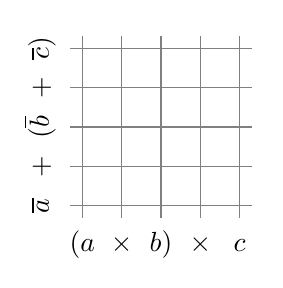
\begin{tikzpicture}[matrix]
                \foreach \x/\a in {1/\dual{\atom1}, 2/\+, 3/(\dual{\atom2}, 4/\+, 5/\dual{\atom3})}%
                    \draw[gray] (\x,0) node[src] {$\a$} (\x,.7) -- (\x,5.3);
                \foreach \y/\b in {1/(\atom1, 2/\*, 3/\atom2), 4/\*, 5/\atom3}%
                    \draw[gray] (0,\y) node[tgt] {$\b$} (.7,\y) -- (5.3,\y);
            \end{tikzpicture}}
            \quad\leadsto\quad
            \vc{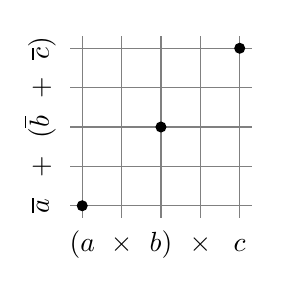
\begin{tikzpicture}[matrix]
                \foreach \x/\a in {1/\dual{\atom1}, 2/\+, 3/(\dual{\atom2}, 4/\+, 5/\dual{\atom3})}%
                    \draw[gray] (\x,0) node[src] {$\a$} (\x,.7) -- (\x,5.3);
                \foreach \y/\b in {1/(\atom1, 2/\*, 3/\atom2), 4/\*, 5/\atom3}%
                    \draw[gray] (0,\y) node[tgt] {$\b$} (.7,\y) -- (5.3,\y);
                \foreach \p/\n in { {1,1}/a1, {3,3}/b1, {5,5}/c1} \node[tokB] (\n) at (\p) {};
            \end{tikzpicture}}
        \]

        \begin{itemize}
            \item See \citet{petri-nets}
            \item Corresponds to axiom rule for ALL
        \end{itemize}

    }

    \frame{
        \frametitle{Coalescence Proof Search}

        Transitions:
        \[
            \begin{array}{ccc}
                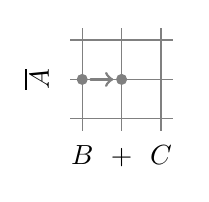
\begin{tikzpicture}[matrix]
                    \foreach \i/\a in {1/{}, 2/\dual A, 3/{}}
                        {\draw[gray] (\i,0) node[src] {$\a$} (\i,.7) -- (\i,3.3);}
                    \foreach \j/\b in {1/B, 2/\+, 3/C}
                        {\draw[gray] (0,\j) node[tgt] {$\b$} (.7,\j) -- (3.3,\j);}
                    \node[tokG] (a) at (2,1) {};
                    \node[tokG] (c) at (2,2) {};
                    \draw[jmp1] (a) to (c);
                \end{tikzpicture}
                &
                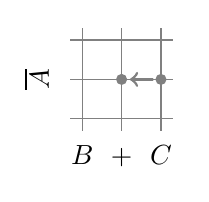
\begin{tikzpicture}[matrix]
                    \foreach \i/\a in {1/{}, 2/\dual A, 3/{}}
                        {\draw[gray] (\i,0) node[src] {$\a$} (\i,.7) -- (\i,3.3);}
                    \foreach \j/\b in {1/B, 2/\+, 3/C}
                        {\draw[gray] (0,\j) node[tgt] {$\b$} (.7,\j) -- (3.3,\j);}
                    \node[tokG] (b) at (2,3) {};
                    \node[tokG] (c) at (2,2) {};
                    \draw[jmp1] (b) to (c);
                \end{tikzpicture}
                &
                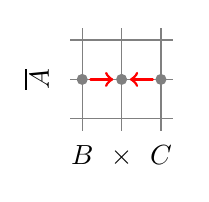
\begin{tikzpicture}[matrix]
                  \foreach \i/\a in {1/{}, 2/\dual A, 3/{}}
                    {\draw[gray] (\i,0) node[src] {$\a$} (\i,.7) -- (\i,3.3);}
                  \foreach \j/\b in {1/B, 2/\*, 3/C}
                    {\draw[gray] (0,\j) node[tgt] {$\b$} (.7,\j) -- (3.3,\j);}
                  \node[tokG] (a) at (2,1) {};
                  \node[tokG] (b) at (2,3) {};
                  \node[tokG] (c) at (2,2) {};
                  \draw[jmp2] (a) to (c);
                  \draw[jmp2] (b) to (c);
                \end{tikzpicture}
                \\
                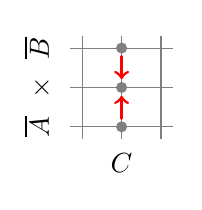
\begin{tikzpicture}[matrix]
                    \foreach \i/\a in {1/\dual A, 2/\*, 3/\dual B}
                        {\draw[gray] (\i,0) node[src] {$\a$} (\i,.7) -- (\i,3.3);}
                    \foreach \j/\b in {1/{}, 2/C, 3/{}}
                        {\draw[gray] (0,\j) node[tgt] {$\b$} (.7,\j) -- (3.3,\j);}
                    \node[tokG] (a) at (1,2) {};
                    \node[tokG] (b) at (3,2) {};
                    \node[tokG] (c) at (2,2) {};
                    \draw[jmp2] (a) to (c);
                    \draw[jmp2] (b) to (c);
                \end{tikzpicture}
                &
                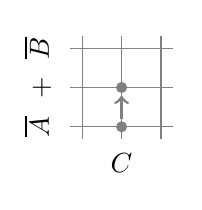
\begin{tikzpicture}[matrix]
                    \foreach \i/\a in {1/\dual A, 2/\+, 3/\dual B}
                        {\draw[gray] (\i,0) node[src] {$\a$} (\i,.7) -- (\i,3.3);}
                    \foreach \j/\b in {1/{}, 2/C, 3/{}}
                        {\draw[gray] (0,\j) node[tgt] {$\b$} (.7,\j) -- (3.3,\j);}
                    \node[tokG] (a) at (1,2) {};
                    \node[tokG] (c) at (2,2) {};
                    \draw[jmp1] (a) to (c);
                \end{tikzpicture}
                &
                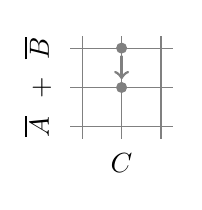
\begin{tikzpicture}[matrix]
                    \foreach \i/\a in {1/\dual A, 2/\+, 3/\dual B}
                        {\draw[gray] (\i,0) node[src] {$\a$} (\i,.7) -- (\i,3.3);}
                    \foreach \j/\b in {1/{}, 2/C, 3/{}}
                        {\draw[gray] (0,\j) node[tgt] {$\b$} (.7,\j) -- (3.3,\j);}
                    \node[tokG] (b) at (3,2) {};
                    \node[tokG] (c) at (2,2) {};
                    \draw[jmp1] (b) to (c);
                \end{tikzpicture}
            \end{array}
        \]
    }

    \frame{
        \frametitle{Coalescence Proof Search}

        Corresponding sequent rules for ALL:
        \[
            \begin{minipage}[H]{\linewidth}
                \centering
                \begin{minipage}[H]{0.3\linewidth}
                    \begin{prooftree}
                        \AxiomC{$\vdash A, B$}
                        \UnaryInfC{$\vdash A, B \+ C$}
                    \end{prooftree}
                \end{minipage}
                \begin{minipage}[H]{0.3\linewidth}
                    \begin{prooftree}
                        \AxiomC{$\vdash A, C$}
                        \UnaryInfC{$\vdash A, B \+ C$}
                    \end{prooftree}
                \end{minipage}
                \begin{minipage}[H]{0.3\linewidth}
                    \begin{prooftree}
                        \AxiomC{$\vdash A, B$}
                        \AxiomC{$\vdash A, C$}
                        \BinaryInfC{$\vdash A, B \* C$}
                    \end{prooftree}
                \end{minipage}
                
                \begin{minipage}[H]{0.3\linewidth}
                    \begin{prooftree}
                        \AxiomC{$\vdash A, C$}
                        \AxiomC{$\vdash B, C$}
                        \BinaryInfC{$\vdash A \* B, C$}
                    \end{prooftree}
                \end{minipage}
                \begin{minipage}[H]{0.3\linewidth}
                    \begin{prooftree}
                        \AxiomC{$\vdash A, C$}
                        \UnaryInfC{$\vdash A \+ B, C$}
                    \end{prooftree}
                \end{minipage}
                \begin{minipage}[H]{0.3\linewidth}
                    \begin{prooftree}
                        \AxiomC{$\vdash B, C$}
                        \UnaryInfC{$\vdash A \+ B, C$}
                    \end{prooftree}
                \end{minipage}
            \end{minipage}
        \]
    }

    \frame{
        \frametitle{Coalescence Proof Search}

        Example:
        \[
            \vc{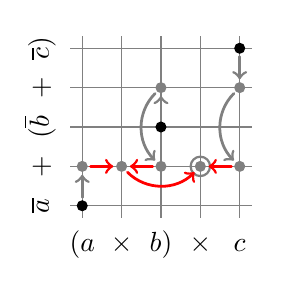
\begin{tikzpicture}[matrix]
                \foreach \x/\a in {1/\dual{\atom1}, 2/\+, 3/(\dual{\atom2}, 4/\+, 5/\dual{\atom3})}%
                    \draw[gray] (\x,0) node[src] {$\a$} (\x,.7) -- (\x,5.3);
                \foreach \y/\b in {1/(\atom1, 2/\*, 3/\atom2), 4/\*, 5/\atom3}%
                    \draw[gray] (0,\y) node[tgt] {$\b$} (.7,\y) -- (5.3,\y);
                \foreach \p/\n in {
                    {2,1}/a2, {2,2}/ab,
                    {4,3}/b2, {2,3}/b3,
                    {4,5}/c2, {2,5}/c3%
                } \node[tokG] (\n) at (\p) {};
                \node[tokG] (abc) at (2,4) {};
                \node[circle,draw,gray,thick,inner sep=0pt,minimum size=7pt] at (2,4) {};
                \foreach \p/\n in { {1,1}/a1, {3,3}/b1, {5,5}/c1} \node[tokB] (\n) at (\p) {};
                \foreach \s/\t in { a1/a2, b1/b2, c1/c2} \draw[jmp1] (\s)--(\t);
                \foreach \s/\t in { a2/ab, b3/ab, c3/abc} \draw[jmp2] (\s)--(\t);
                \draw[jmp1,bend right=45] (b2) to (b3);
                \draw[jmp1,bend right=45] (c2) to (c3);
                \draw[jmp2,bend right=45] (ab) to (abc);
            \end{tikzpicture}}
        \]
    }



    \frame{
        \frametitle{Classical Logic (CL)}

        \[
            A, B, C \quad \defeq \quad \top \mid \bot \mid a \mid \dual a \mid A \vee B \mid A \wedge B
        \]

        \begin{itemize}
            \item $\bot, \atom1, \vee$ are duals of $\top, \dual{\atom1}, \wedge$
            \item Similar to ALL formulae
        \end{itemize}
    }

    \frame{
        \frametitle{Classical Logic (CL)}

        Examples:
        \begin{itemize}
            \item $(\atom1 \vee \dual{\atom1}) \wedge (\atom2 \vee \dual{\atom2})$ will be a recurrent example
            \item $\dual{\atom1 \vee \dual{\atom2}} \leftrightsquigarrow \dual{\atom1} \wedge \atom2$ and associated De Morgan laws
            \item $\dual{A} \vee B \leftrightsquigarrow A \implies B$ and other useful syntax
        \end{itemize}
    }

    \frame{
        \frametitle{Classical Logic (CL)}
        
        Sequent calculus with \emph{additive} rules:
        \begin{figure}[H]
            \centering
            \begin{minipage}[H]{.3\linewidth}
                \begin{prooftree}
                    \AxiomC{~}
                    \RightLabel{$\top$}
                    \UnaryInfC{$\vdash \top$}
                \end{prooftree}
            \end{minipage}
            \begin{minipage}[H]{.3\linewidth}
                \begin{prooftree}
                    \AxiomC{$\vdash \Gamma, A$}
                    \RightLabel{$\vee$}
                    \UnaryInfC{$\vdash \Gamma, A \vee B$}
                \end{prooftree}
            \end{minipage}
            \begin{minipage}[H]{.3\linewidth}
                \begin{prooftree}
                    \AxiomC{$\vdash \Gamma$}
                    \RightLabel{$w$}
                    \UnaryInfC{$\vdash \Gamma, A$}
                \end{prooftree}
            \end{minipage}

            \begin{minipage}[H]{.3\linewidth}
                \begin{prooftree}
                    \AxiomC{~}
                    \RightLabel{$ax$}
                    \UnaryInfC{$\vdash a, \dual a$}
                \end{prooftree}
            \end{minipage}
            \begin{minipage}[H]{.3\linewidth}
                \begin{prooftree}
                    \AxiomC{$\vdash \Gamma, A$}
                    \AxiomC{$\vdash \Gamma, B$}
                    \RightLabel{$\wedge$}
                    \BinaryInfC{$\vdash \Gamma, A \wedge B$}
                \end{prooftree}
            \end{minipage}
            \begin{minipage}[H]{.3\linewidth}
                \begin{prooftree}
                    \AxiomC{$\vdash \Gamma, A, A$}
                    \RightLabel{$c$}
                    \UnaryInfC{$\vdash \Gamma, A$}
                \end{prooftree}
            \end{minipage}
        \end{figure}

        \begin{itemize}
            \item $A, B, C$ are formulae, $\Gamma, \Delta, \Sigma$ are sequents
            \item $\wedge, \vee$ rules preserve the number of terms in a sequent, $c, w$ rules do not
            \item Sequents are commutative, \emph{morally equivalent} up to idempotence
        \end{itemize}
    }

    \frame{
        \frametitle{Classical Logic (CL)}

        Example:
        \begin{prooftree}
            \AxiomC{$~$}
            \RightLabel{$ax$}\UnaryInfC{$\vdash \atom1, \neg \atom1$}
            \RightLabel{$\vee$}\UnaryInfC{$\vdash \atom1 \vee \neg \atom1, \neg \atom1$}
            \RightLabel{$\vee$}\UnaryInfC{$\vdash \atom1 \vee \neg \atom1, \atom1 \vee \neg \atom1$}
            \RightLabel{$c$}\UnaryInfC{$\vdash \atom1 \vee \neg \atom1$}
            \AxiomC{$~$}
            \RightLabel{$\top$}\UnaryInfC{$\vdash \top$}
            \RightLabel{$\wedge$}\BinaryInfC{$\vdash (\atom1 \vee \neg \atom1) \wedge \top$}
        \end{prooftree}
    }



    \frame{
        \frametitle{Additive Stratification}

        \begin{prooftree}
            \AxiomC{}
            \RightLabel{$\top, ax$}\doubleLine\UnaryInfC{$\vdash A_1$}
            \RightLabel{$w$}\doubleLine\UnaryInfC{$\vdash \Gamma_1$}
            \AxiomC{\dots}
            \AxiomC{}
            \RightLabel{$\top, ax$}\doubleLine\UnaryInfC{$\vdash A_n$}
            \RightLabel{$w$}\doubleLine\UnaryInfC{$\vdash \Gamma_n$}
            \RightLabel{$\wedge, \vee$}\doubleLine\TrinaryInfC{$\vdash P \dots P$}
            \RightLabel{$c$}\doubleLine\UnaryInfC{$\vdash P$}
        \end{prooftree}
        \begin{itemize}
            \item Does not work for \emph{multiplicative} $\vee, \wedge$ rules, see \citet{contraction-restrictions}
        \end{itemize}
    }

    \frame{
        \frametitle{Additive Stratification}

        \begin{figure}[H]
            \centering
            \begin{minipage}[H]{0.4\linewidth}
                \begin{prooftree}
                    \AxiomC{$\vdash \Gamma, A$}
                    \RightLabel{$\vee$}\UnaryInfC{$\vdash \Gamma, A \vee B$}
                    \RightLabel{$w$}\UnaryInfC{$\vdash \Gamma, A \vee B$, C}
                \end{prooftree}
            \end{minipage}
            $\leadsto$
            \begin{minipage}[H]{0.4\linewidth}
                \begin{prooftree}
                    \AxiomC{$\vdash \Gamma, A$}
                    \RightLabel{$w$}\UnaryInfC{$\vdash \Gamma, A, C$}
                    \RightLabel{$\vee$}\UnaryInfC{$\vdash \Gamma, A \vee B, C$}
                \end{prooftree}
            \end{minipage}
        \end{figure}
        
        \begin{figure}[H]
            \centering
            \begin{minipage}[H]{0.4\linewidth}
                \begin{prooftree}
                    \AxiomC{$\vdash \Gamma, A$}
                    \AxiomC{$\vdash \Gamma, B$}
                    \RightLabel{$\wedge$}\BinaryInfC{$\vdash \Gamma, A \wedge B$}
                    \RightLabel{$w$}\UnaryInfC{$\vdash \Gamma, A \wedge B, C$}
                \end{prooftree}
            \end{minipage}
            $\leadsto\quad$
            \begin{minipage}[H]{0.4\linewidth}
                \begin{prooftree}
                    \AxiomC{$\vdash \Gamma, A$}
                    \RightLabel{$w$}\UnaryInfC{$\vdash \Gamma, A, C$}
                    \AxiomC{$\vdash \Gamma, B$}
                    \RightLabel{$w$}\UnaryInfC{$\vdash \Gamma, B, C$}
                    \RightLabel{$\wedge$}\BinaryInfC{$\vdash \Gamma, A \wedge B, C$}
                \end{prooftree}
            \end{minipage}
        \end{figure}

        \begin{figure}[H]
            \centering
            \begin{minipage}[H]{0.4\linewidth}
                \begin{prooftree}
                    \AxiomC{$\vdash \Gamma, A, A$}
                    \RightLabel{$c$}\UnaryInfC{$\vdash \Gamma, A$}
                    \RightLabel{$w$}\UnaryInfC{$\vdash \Gamma, A, B$}
                \end{prooftree}
            \end{minipage}
            $\leadsto\quad$
            \begin{minipage}[H]{0.4\linewidth}
                \begin{prooftree}
                    \AxiomC{$\vdash \Gamma, A, A$}
                    \RightLabel{$w$}\UnaryInfC{$\vdash \Gamma, A, A, B$}
                    \RightLabel{$c$}\UnaryInfC{$\vdash \Gamma, A, B$}
                \end{prooftree}
            \end{minipage}
        \end{figure}
    }

    \frame{
        \frametitle{Additive Stratification}

        \begin{figure}[H]
            \centering
            \begin{minipage}[H]{0.4\linewidth}
                \begin{prooftree}
                    \AxiomC{$\vdash \Gamma, A, A$}
                    \RightLabel{$c$}\UnaryInfC{$\vdash \Gamma, A$}
                    \RightLabel{$\vee$}\UnaryInfC{$\vdash \Gamma, A \vee B$}
                \end{prooftree}
            \end{minipage}
            $\leadsto$
            \begin{minipage}[H]{0.4\linewidth}
                \begin{prooftree}
                    \AxiomC{$\vdash \Gamma, A, A$}
                    \RightLabel{$\vee$}\UnaryInfC{$\vdash \Gamma, A \vee B, A$}
                    \RightLabel{$\vee$}\UnaryInfC{$\vdash \Gamma, A \vee B, A \vee B$}
                    \RightLabel{$c$}\UnaryInfC{$\vdash \Gamma, A \vee B$}
                \end{prooftree}
            \end{minipage}
        \end{figure}

        \begin{figure}[H]
            \centering
            \begin{minipage}[H]{0.3\linewidth}
                \begin{scprooftree}{0.8}
                    \AxiomC{$\vdash \Gamma, A, A$}
                    \RightLabel{$c$}\UnaryInfC{$\vdash \Gamma, A$}
                    \AxiomC{$\vdash \Gamma, B$}
                    \RightLabel{$\wedge$}\BinaryInfC{$\vdash \Gamma, A \wedge B$}
                \end{scprooftree}
            \end{minipage}
            $\leadsto\quad$
            \begin{minipage}[H]{0.6\linewidth}
                \begin{scprooftree}{0.8}
                    \AxiomC{$\vdash \Gamma, A, A$}
                    \AxiomC{$\vdash \Gamma, B$}
                    \RightLabel{$w$}\UnaryInfC{$\vdash \Gamma, A, B$}
                    \RightLabel{$\wedge$}\BinaryInfC{$\vdash \Gamma, A, A \wedge B$}
                    \AxiomC{$\vdash \Gamma, B$}
                    \RightLabel{$w$}\UnaryInfC{$\vdash \Gamma, B, A \wedge B$}
                    \RightLabel{$\wedge$}\BinaryInfC{$\vdash \Gamma, A \wedge B, A \wedge B$}
                    \RightLabel{$c$}\UnaryInfC{$\vdash \Gamma, A \wedge B$}
                \end{scprooftree}
            \end{minipage}
        \end{figure}
    }

    \frame{
        \frametitle{Additive Stratification}

        Previous Example:
        \begin{prooftree}
            \AxiomC{$~$}
            \RightLabel{$ax$}\UnaryInfC{$\vdash \atom1, \neg \atom1$}
            \RightLabel{$\vee$}\UnaryInfC{$\vdash \atom1 \vee \neg \atom1, \neg \atom1$}
            \RightLabel{$\vee$}\UnaryInfC{$\vdash \atom1 \vee \neg \atom1, \atom1 \vee \neg \atom1$}
            \RightLabel{$c$}\UnaryInfC{$\vdash \atom1 \vee \neg \atom1$}
            \AxiomC{$~$}
            \RightLabel{$\top$}\UnaryInfC{$\vdash \top$}
            \RightLabel{$\wedge$}\BinaryInfC{$\vdash (\atom1 \vee \neg \atom1) \wedge \top$}
        \end{prooftree}
    }

    \frame{
        \frametitle{Additive Stratification}

        Example:
        \begin{prooftree}
            \AxiomC{$~$}
            \RightLabel{$ax$}\UnaryInfC{$\vdash \atom1, \neg \atom1$}
            \RightLabel{$\vee$}\UnaryInfC{$\vdash \atom1 \vee \neg \atom1, \neg \atom1$}
            \RightLabel{$\vee$}\UnaryInfC{$\vdash \atom1 \vee \neg \atom1, \atom1 \vee \neg \atom1$}
            \AxiomC{$~$}
            \RightLabel{$\top$}\UnaryInfC{$\vdash \top$}
            \RightLabel{$w$}\UnaryInfC{$\vdash \top, \atom1 \vee \neg \atom1$}
            \RightLabel{$\wedge$}\BinaryInfC{$\vdash (\atom1 \vee \neg \atom1) \wedge \top, \atom1 \vee \neg \atom1$}
            \AxiomC{$~$}
            \RightLabel{$\top$}\UnaryInfC{$\vdash \top$}
            \RightLabel{$w$}\UnaryInfC{$\vdash (\atom1 \vee \neg \atom1) \wedge \top, \top$}
            \RightLabel{$\wedge$}\BinaryInfC{$\vdash (\atom1 \vee \neg \atom1) \wedge \top, (\atom1 \vee \neg \atom1) \wedge \top$}
            \RightLabel{$c$}\UnaryInfC{$\vdash (\atom1 \vee \neg \atom1) \wedge \top$}
        \end{prooftree}
    }



    \frame{
        \frametitle{Coalescence Proof Search in CL}

        \begin{itemize}
            \item No longer polynomially bounded
            \item Coalescence on $|A|^n$
            \item Increase $n$ until \dots ?
        \end{itemize}
    }

    \frame{
        \frametitle{Coalescence Proof Search in CL}

        Example: $\bot \vee (\top \wedge \top)$, $n \seteq 1$

        \newcommand\spawnIGrid[1]{\vc{\begin{tikzpicture}[matrix,x=-3.5mm,y=3.5mm]
                \foreach \x/\a in {1/\,} \draw[gray] (\x,0) node[src] {\footnotesize$\a$} (\x,.7) -- (\x,5.3);
                \foreach \y/\b in {1/\bot, 2/\vee, 3/\top, 4/\wedge, 5/\top} \draw[gray] (0,\y) node[tgt] {\footnotesize$\b$} (.7,\y) -- (1.3,\y);
                \foreach \p/\n/\c in {####1} \node[fill,tok,\c] (\n) at (\p) {};
            \end{tikzpicture}}}
        \newcommand\initSpawnIGrid{\spawnIGrid{{1,3}/a1/blue, {1,5}/b1/red}}

        \[
             \initSpawnIGrid
             \quad\leadsto\quad
             \spawnIGrid{{1,3}/a1/blue, {1,5}/b1/red, {1,4}/c1/purple}
             \quad\leadsto\quad
             \spawnIGrid{{1,3}/a1/blue, {1,5}/b1/red, {1,4}/c1/purple, {1,2}/d1/purple}
        \]

    }

    \frame{
        \frametitle{Coalescence Proof Search in CL}

        Example: $\atom1 \vee \dual{\atom1}$, $n \seteq 2$

        \newcommand\spawnIIGrid[1]{\vc{\begin{tikzpicture}[matrix,x=-3.5mm,y=3.5mm]
                \foreach \x/\a in {1/\atom1, 2/\vee, 3/\dual{\atom1}} \draw[gray] (\x,0) node[src] {\footnotesize$\a$} (\x,.7) -- (\x,3.3);
                \foreach \y/\b in {1/\atom1, 2/\vee, 3/\dual{\atom1}} \draw[gray] (0,\y) node[tgt] {\footnotesize$\b$} (.7,\y) -- (3.3,\y);
                \foreach \p/\n/\c in {####1} \node[fill,tok,\c] (\n) at (\p) {};
            \end{tikzpicture}}}
        \newcommand\initSpawnIIGrid{\spawnIIGrid{{1,3}/a1/blue, {3,1}/b1/red}}

        \[
             \initSpawnIIGrid
             \quad\leadsto\quad
             \spawnIIGrid{{1,3}/a1/blue, {3,1}/b1/red, {2,3}/c1/blue}
             \quad\leadsto\quad
             \spawnIIGrid{{1,3}/a1/blue, {3,1}/b1/red, {2,3}/c1/blue, {3,2}/d1/red}
             \quad\leadsto\quad
             \spawnIIGrid{{1,3}/a1/blue, {3,1}/b1/red, {2,3}/c1/blue, {3,2}/d1/red, {2,2}/e1/blue}
        \]
    
    }

    \frame{
        \frametitle{Coalescence Proof Search in CL}

        Example $(\atom1 \vee \dual{\atom1}) \wedge (\atom2 \vee \dual{\atom2})$, $n \seteq 2$ 

        \newcommand\spawnIIGrid[1]{\vc{\begin{tikzpicture}[matrix,x=-3.5mm,y=3.5mm]
                \foreach \x/\a in {1/\atom1, 2/\vee, 3/\dual{\atom1}, 4/\wedge, 5/\atom2, 6/\vee, 7/\dual{\atom2}} \draw[gray] (\x,0) node[src] {\footnotesize$\a$} (\x,.7) -- (\x,7.3);
                \foreach \y/\b in {1/\atom1, 2/\vee, 3/\dual{\atom1}, 4/\wedge, 5/\atom2, 6/\vee, 7/\dual{\atom2}} \draw[gray] (0,\y) node[tgt] {\footnotesize$\b$} (.7,\y) -- (7.3,\y);
                \foreach \p/\n/\c in {####1} \node[fill,tok,\c] (\n) at (\p) {};
            \end{tikzpicture}}}
        \newcommand\initSpawnIIGrid{\spawnIIGrid{{1,3}/a1/blue, {3,1}/b1/black!10!green, {5,7}/c1/red, {7,5}/d1/black!10!yellow}}

        \[
            \initSpawnIIGrid
            \quad\leadsto^*\quad
            \spawnIIGrid{{1,3}/a1/blue, {2,3}/a2/blue, {1,2}/a3/blue, {2,2}/a4/blue, {3,1}/b1/black!10!green, {3,2}/b2/black!10!green, {2,1}/b3/black!10!green, {5,7}/c1/red, {6,7}/c2/red, {5,6}/c3/red, {6,6}/c4/red, {7,5}/d1/black!10!yellow, {7,6}/d2/black!10!yellow, {6,5}/d3/black!10!yellow}
        \]
    }

    \frame{
        \frametitle{Coalescence Proof Search in CL}

        Example $(\atom1 \vee \dual{\atom1}) \wedge (\atom2 \vee \dual{\atom2})$, $n \seteq 3$, $A \seteq \atom1 \vee \dual{\atom1}$, $B \seteq \atom2 \vee \dual{\atom2}$
        
        \begin{minipage}{\linewidth}
            \centering
            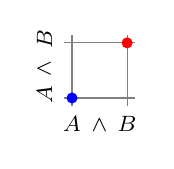
\begin{tikzpicture}[matrix,x=-3.5mm,y=3.5mm]
                \foreach \xs/\ys/\xz/\yz/\xl/\yl/\rot in {0/0/1/0/0/2/90, 0/0/0/1/2/0/0} {
                    \foreach \z/\a/\d in {0/A/1, 1/\wedge/0, 2/B/1}
                        \ifthenelse{\d = 0}{
                            \draw[gray] (\xs + \z*\xz - \xl*0.5, \ys + \z*\yz - \yl*0.5)
                                node[tgt] {\ifthenelse{\rot > -1}{\rotatebox{\rot}{\footnotesize$\a$}}{}}
                                (0,0) -- (0,0)}{
                            \draw[gray] (\xs + \z*\xz - \xl*0.5, \ys + \z*\yz - \yl*0.5)
                                node[tgt] {\ifthenelse{\rot > -1}{\rotatebox{\rot}{\footnotesize$\a$}}{}}
                                (\xs + \z*\xz - \xl*0.15, \ys + \z*\yz - \yl*0.15) -- (\xs + \z*\xz + \xl*1.15, \ys + \z*\yz + \yl*1.15)};};
                \foreach \p/\n/\d in {{0,0}/a1/blue, {2,2}/b1/red} \node[fill,tok,\d] (\n) at (\p) {};
            \end{tikzpicture}

            \begin{minipage}[H]{0.18\linewidth}
                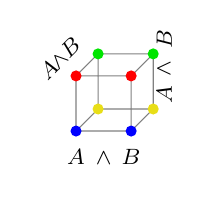
\begin{tikzpicture}[matrix,x=-3.5mm,y=3.5mm]
                    \foreach \xs/\ys/\xz/\yz/\xl/\yl/\rot in {0/0/0/1/2/0/0, 0.8/2.8/1/0/-.8/-.8/90, 2/0/.4/.4/0/2/45} {
                        \foreach \z/\a/\d in {0/A/1, 1/\wedge/0, 2/B/1} \draw[gray] (\xs + \z*\xz - \xl*0.5, \ys + \z*\yz - \yl*0.5) node[tgt] {\ifthenelse{\rot > -1}{\rotatebox{\rot}{\footnotesize$\a$}}{}} (0,0) -- (0,0);}
                    \draw[gray] (0,0) -- (2,0) -- (2,2) -- (0,2) -- (0,0) -- (.8,.8) -- (2.8,.8) -- (2.8,2.8) -- (.8,2.8) -- (.8,.8) -- (2.8,.8) -- (2,0) -- (2,2) -- (2.8,2.8) -- (.8,2.8) -- (0,2);
                    \foreach \s/\e/\n/\d in {{0,0}/{0,2}/a1/blue, {2,0}/{2,2}/b1/red, {2.8,.8}/{2.8,2.8}/c1/black!10!green, {.8,.8}/{.8,2.8}/d1/black!10!yellow} {
                        \node[fill,tok,\d] (\n) at (\s) {};
                        \node[fill,tok,\d] (\n) at (\e) {};}
                \end{tikzpicture}
            \end{minipage}
            $\leadsto^*$
            \begin{minipage}[H]{0.18\linewidth}
                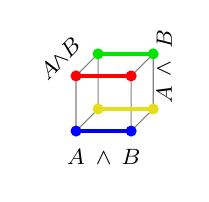
\begin{tikzpicture}[matrix,x=-3.5mm,y=3.5mm]
                    \foreach \xs/\ys/\xz/\yz/\xl/\yl/\rot in {0/0/0/1/2/0/0, 0.8/2.8/1/0/-.8/-.8/90, 2/0/.4/.4/0/2/45} {
                        \foreach \z/\a/\d in {0/A/1, 1/\wedge/0, 2/B/1} \draw[gray] (\xs + \z*\xz - \xl*0.5, \ys + \z*\yz - \yl*0.5) node[tgt] {\ifthenelse{\rot > -1}{\rotatebox{\rot}{\footnotesize$\a$}}{}} (0,0) -- (0,0);}
                    \draw[gray] (0,0) -- (2,0) -- (2,2) -- (0,2) -- (0,0) -- (.8,.8) -- (2.8,.8) -- (2.8,2.8) -- (.8,2.8) -- (.8,.8) -- (2.8,.8) -- (2,0) -- (2,2) -- (2.8,2.8) -- (.8,2.8) -- (0,2);
                    \foreach \s/\e/\n/\d in {{0,0}/{0,2}/a1/blue, {2,0}/{2,2}/b1/red, {2.8,.8}/{2.8,2.8}/c1/black!10!green, {.8,.8}/{.8,2.8}/d1/black!10!yellow} {
                        \node[fill,tok,\d] (\n) at (\s) {};
                        \node[fill,tok,\d] (\n) at (\e) {};
                        \draw[very thick,fill,tok,\d] (\s) -- (\e);}
                \end{tikzpicture}
            \end{minipage}
            $\leadsto^*$
            \begin{minipage}[H]{0.18\linewidth}
                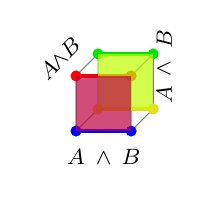
\begin{tikzpicture}[matrix,x=-3.5mm,y=3.5mm]
                    \foreach \xs/\ys/\xz/\yz/\xl/\yl/\rot in {0/0/0/1/2/0/0, 0.8/2.8/1/0/-.8/-.8/90, 2/0/.4/.4/0/2/45} {
                        \foreach \z/\a/\d in {0/A/1, 1/\wedge/0, 2/B/1} \draw[gray] (\xs + \z*\xz - \xl*0.5, \ys + \z*\yz - \yl*0.5) node[tgt] {\ifthenelse{\rot > -1}{\rotatebox{\rot}{\footnotesize$\a$}}{}} (0,0) -- (0,0);}
                    \draw[gray] (0,0) -- (2,0) -- (2,2) -- (0,2) -- (0,0) -- (.8,.8) -- (2.8,.8) -- (2.8,2.8) -- (.8,2.8) -- (.8,.8) -- (2.8,.8) -- (2,0) -- (2,2) -- (2.8,2.8) -- (.8,2.8) -- (0,2);
                    \foreach \s/\e/\n/\d in {{0,0}/{0,2}/a1/blue, {2,0}/{2,2}/b1/red, {2.8,.8}/{2.8,2.8}/c1/black!10!green, {.8,.8}/{.8,2.8}/d1/black!10!yellow} {
                        \node[fill,tok,\d] (\n) at (\s) {};
                        \node[fill,tok,\d] (\n) at (\e) {};
                        \draw[very thick,tok,\d] (\s) -- (\e);}
                    \fill[tok,fill=lime,opacity=.7] (2.8,.8) rectangle (.8,2.8);
                    \fill[tok,fill=purple,opacity=.7] (0,0) rectangle (2,2);
                \end{tikzpicture}
            \end{minipage}
            $\leadsto$
            \begin{minipage}[H]{0.18\linewidth}
                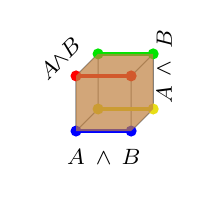
\begin{tikzpicture}[matrix,x=-3.5mm,y=3.5mm]
                    \foreach \xs/\ys/\xz/\yz/\xl/\yl/\rot in {0/0/0/1/2/0/0, 0.8/2.8/1/0/-.8/-.8/90, 2/0/.4/.4/0/2/45} {
                        \foreach \z/\a/\d in {0/A/1, 1/\wedge/0, 2/B/1} \draw[gray] (\xs + \z*\xz - \xl*0.5, \ys + \z*\yz - \yl*0.5) node[tgt] {\ifthenelse{\rot > -1}{\rotatebox{\rot}{\footnotesize$\a$}}{}} (0,0) -- (0,0);}
                    \draw[gray] (0,0) -- (2,0) -- (2,2) -- (0,2) -- (0,0) -- (.8,.8) -- (2.8,.8) -- (2.8,2.8) -- (.8,2.8) -- (.8,.8) -- (2.8,.8) -- (2,0) -- (2,2) -- (2.8,2.8) -- (.8,2.8) -- (0,2);
                    \foreach \s/\e/\n/\d in {{0,0}/{0,2}/a1/blue, {2,0}/{2,2}/b1/red, {2.8,.8}/{2.8,2.8}/c1/black!10!green, {.8,.8}/{.8,2.8}/d1/black!10!yellow} {
                        \node[fill,tok,\d] (\n) at (\s) {};
                        \node[fill,tok,\d] (\n) at (\e) {};
                        \draw[very thick,tok,\d] (\s) -- (\e);}
                    \fill[tok,fill=brown,opacity=.7] (0,0) -- (0,2) -- (.8,2.8) -- (2.8,2.8) -- (2.8,.8) -- (2,0) -- cycle;
                \end{tikzpicture}
            \end{minipage}
        \end{minipage}
    }



    \frame{
        \frametitle{Dimensionality}
		
		\begin{align*}
			\mathcal{D}^1 \quad &\defeq \quad \top \mid \bot \mid \mathcal{D}^1 \vee \mathcal{D}^1 \mid \mathcal{D}^1 \wedge \mathcal{D}^1 \\
			\mathcal{D}^2 \quad &\defeq \quad ALL \\
				      &\dots
		\end{align*}

		\begin{itemize}
			\item Difficult to categorise further
			\item Unsatisfactory results for $(a \vee \dual a) \wedge \dots \wedge (z \vee \dual z)$
		\end{itemize}
    }



    \frame{
        \frametitle{Satisfying Optimisations}
        
        \begin{minipage}[H]{\linewidth}
            \centering
            \begin{minipage}[H]{0.15\linewidth}
                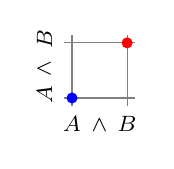
\begin{tikzpicture}[matrix,x=-3.5mm,y=3.5mm]
                    \foreach \xs/\ys/\xz/\yz/\xl/\yl/\rot in {0/0/1/0/0/2/90, 0/0/0/1/2/0/0} {
                        \foreach \z/\a/\d in {0/A/1, 1/\wedge/0, 2/B/1}
                            \ifthenelse{\d = 0}{
                                \draw[gray] (\xs + \z*\xz - \xl*0.5, \ys + \z*\yz - \yl*0.5)
                                    node[tgt] {\ifthenelse{\rot > -1}{\rotatebox{\rot}{\footnotesize$\a$}}{}}
                                    (0,0) -- (0,0)}{
                                \draw[gray] (\xs + \z*\xz - \xl*0.5, \ys + \z*\yz - \yl*0.5)
                                    node[tgt] {\ifthenelse{\rot > -1}{\rotatebox{\rot}{\footnotesize$\a$}}{}}
                                    (\xs + \z*\xz - \xl*0.15, \ys + \z*\yz - \yl*0.15) -- (\xs + \z*\xz + \xl*1.15, \ys + \z*\yz + \yl*1.15)};};
                    \foreach \p/\n/\d in {{0,0}/a1/blue, {2,2}/b1/red} \node[fill,tok,\d] (\n) at (\p) {};
                \end{tikzpicture}
            \end{minipage}
            
            \vspace{1cm}

            \begin{minipage}[H]{0.15\linewidth}
                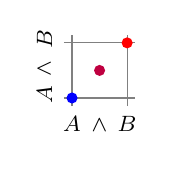
\begin{tikzpicture}[matrix,x=-3.5mm,y=3.5mm]
                    \foreach \xs/\ys/\xz/\yz/\xl/\yl/\rot in {0/0/1/0/0/2/90, 0/0/0/1/2/0/0} {
                        \foreach \z/\a/\d in {0/A/1, 1/\wedge/0, 2/B/1}
                            \ifthenelse{\d = 0}{
                                \draw[gray] (\xs + \z*\xz - \xl*0.5, \ys + \z*\yz - \yl*0.5)
                                    node[tgt] {\ifthenelse{\rot > -1}{\rotatebox{\rot}{\footnotesize$\a$}}{}}
                                    (0,0) -- (0,0)}{
                                \draw[gray] (\xs + \z*\xz - \xl*0.5, \ys + \z*\yz - \yl*0.5)
                                    node[tgt] {\ifthenelse{\rot > -1}{\rotatebox{\rot}{\footnotesize$\a$}}{}}
                                    (\xs + \z*\xz - \xl*0.15, \ys + \z*\yz - \yl*0.15) -- (\xs + \z*\xz + \xl*1.15, \ys + \z*\yz + \yl*1.15)};};
                    \foreach \p/\n/\d in {{0,0}/a1/blue, {2,2}/b1/red, {1,1/c1/purple}} \node[fill,tok,\d] (\n) at (\p) {};
                \end{tikzpicture}
            \end{minipage}
            $\qquad$
            \begin{minipage}[H]{0.15\linewidth}
                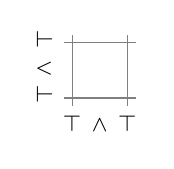
\begin{tikzpicture}[matrix,x=-3.5mm,y=3.5mm]
                    \foreach \xs/\ys/\xz/\yz/\xl/\yl/\rot in {0/0/1/0/0/2/90, 0/0/0/1/2/0/0} {
                        \foreach \z/\a/\d in {0/\top/1, 1/\wedge/0, 2/\top/1}
                            \ifthenelse{\d = 0}{
                                \draw[gray] (\xs + \z*\xz - \xl*0.5, \ys + \z*\yz - \yl*0.5)
                                    node[tgt] {\ifthenelse{\rot > -1}{\rotatebox{\rot}{\footnotesize$\a$}}{}}
                                    (0,0) -- (0,0)}{
                                \draw[gray] (\xs + \z*\xz - \xl*0.5, \ys + \z*\yz - \yl*0.5)
                                    node[tgt] {\ifthenelse{\rot > -1}{\rotatebox{\rot}{\footnotesize$\a$}}{}}
                                    (\xs + \z*\xz - \xl*0.15, \ys + \z*\yz - \yl*0.15) -- (\xs + \z*\xz + \xl*1.15, \ys + \z*\yz + \yl*1.15)};};
                \end{tikzpicture}
            \end{minipage}
            $\leadsto$
            \begin{minipage}[H]{0.15\linewidth}
                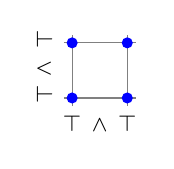
\begin{tikzpicture}[matrix,x=-3.5mm,y=3.5mm]
                    \foreach \xs/\ys/\xz/\yz/\xl/\yl/\rot in {0/0/1/0/0/2/90, 0/0/0/1/2/0/0} {
                        \foreach \z/\a/\d in {0/\top/1, 1/\wedge/0, 2/\top/1}
                            \ifthenelse{\d = 0}{
                                \draw[gray] (\xs + \z*\xz - \xl*0.5, \ys + \z*\yz - \yl*0.5)
                                    node[tgt] {\ifthenelse{\rot > -1}{\rotatebox{\rot}{\footnotesize$\a$}}{}}
                                    (0,0) -- (0,0)}{
                                \draw[gray] (\xs + \z*\xz - \xl*0.5, \ys + \z*\yz - \yl*0.5)
                                    node[tgt] {\ifthenelse{\rot > -1}{\rotatebox{\rot}{\footnotesize$\a$}}{}}
                                    (\xs + \z*\xz - \xl*0.15, \ys + \z*\yz - \yl*0.15) -- (\xs + \z*\xz + \xl*1.15, \ys + \z*\yz + \yl*1.15)};};
                    \foreach \p/\n/\d in {{0,0}/a1/blue, {0,2}/a2/blue, {2,0}/a3/blue, {2,2}/a4/blue} \node[fill,tok,\d] (\n) at (\p) {};
                \end{tikzpicture}
            \end{minipage}
        \end{minipage}
    }


    
    \frame{
        \frametitle{Questions}
         
        \begin{itemize}
            \item Upper bound on dimensionality?
            \begin{itemize}
                \item Exact or approximate?
            \end{itemize}
            \item Good datatype representation for:
            \begin{itemize}
                \item Matrix?
                \item Tokens?
            \end{itemize}
        \end{itemize}
    }



    \frame{
        \frametitle{Datatypes}
        
        \begin{minipage}[H]{\linewidth}
            \centering
            \begin{minipage}[H]{0.15\linewidth}
				\centering
				Tuple:
	
                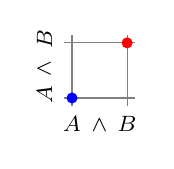
\begin{tikzpicture}[matrix,x=-3.5mm,y=3.5mm]
                    \foreach \xs/\ys/\xz/\yz/\xl/\yl/\rot in {0/0/1/0/0/2/90, 0/0/0/1/2/0/0} {
                        \foreach \z/\a/\d in {0/A/1, 1/\wedge/0, 2/B/1}
                            \ifthenelse{\d = 0}{
                                \draw[gray] (\xs + \z*\xz - \xl*0.5, \ys + \z*\yz - \yl*0.5)
                                    node[tgt] {\ifthenelse{\rot > -1}{\rotatebox{\rot}{\footnotesize$\a$}}{}}
                                    (0,0) -- (0,0)}{
                                \draw[gray] (\xs + \z*\xz - \xl*0.5, \ys + \z*\yz - \yl*0.5)
                                    node[tgt] {\ifthenelse{\rot > -1}{\rotatebox{\rot}{\footnotesize$\a$}}{}}
                                    (\xs + \z*\xz - \xl*0.15, \ys + \z*\yz - \yl*0.15) -- (\xs + \z*\xz + \xl*1.15, \ys + \z*\yz + \yl*1.15)};};
                    \foreach \p/\n/\d in {{0,0}/a1/blue, {2,2}/b1/red} \node[fill,tok,\d] (\n) at (\p) {};
                \end{tikzpicture}
            \end{minipage}
            
            \vspace{1cm}

            \begin{minipage}[H]{0.15\linewidth}
				\centering
				Set:

                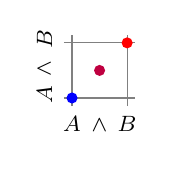
\begin{tikzpicture}[matrix,x=-3.5mm,y=3.5mm]
                    \foreach \xs/\ys/\xz/\yz/\xl/\yl/\rot in {0/0/1/0/0/2/90, 0/0/0/1/2/0/0} {
                        \foreach \z/\a/\d in {0/A/1, 1/\wedge/0, 2/B/1}
                            \ifthenelse{\d = 0}{
                                \draw[gray] (\xs + \z*\xz - \xl*0.5, \ys + \z*\yz - \yl*0.5)
                                    node[tgt] {\ifthenelse{\rot > -1}{\rotatebox{\rot}{\footnotesize$\a$}}{}}
                                    (0,0) -- (0,0)}{
                                \draw[gray] (\xs + \z*\xz - \xl*0.5, \ys + \z*\yz - \yl*0.5)
                                    node[tgt] {\ifthenelse{\rot > -1}{\rotatebox{\rot}{\footnotesize$\a$}}{}}
                                    (\xs + \z*\xz - \xl*0.15, \ys + \z*\yz - \yl*0.15) -- (\xs + \z*\xz + \xl*1.15, \ys + \z*\yz + \yl*1.15)};};
                    \foreach \p/\n/\d in {{0,0}/a1/blue, {2,2}/b1/red, {1,1/c1/purple}} \node[fill,tok,\d] (\n) at (\p) {};
                \end{tikzpicture}
            \end{minipage}
			$\qquad$
			\begin{minipage}[H]{0.35\linewidth}
				\centering
				Multiset:

				\begin{minipage}[H]{0.4\linewidth}
					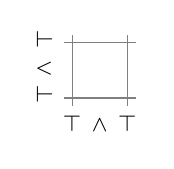
\begin{tikzpicture}[matrix,x=-3.5mm,y=3.5mm]
						\foreach \xs/\ys/\xz/\yz/\xl/\yl/\rot in {0/0/1/0/0/2/90, 0/0/0/1/2/0/0} {
							\foreach \z/\a/\d in {0/\top/1, 1/\wedge/0, 2/\top/1}
								\ifthenelse{\d = 0}{
									\draw[gray] (\xs + \z*\xz - \xl*0.5, \ys + \z*\yz - \yl*0.5)
										node[tgt] {\ifthenelse{\rot > -1}{\rotatebox{\rot}{\footnotesize$\a$}}{}}
										(0,0) -- (0,0)}{
									\draw[gray] (\xs + \z*\xz - \xl*0.5, \ys + \z*\yz - \yl*0.5)
										node[tgt] {\ifthenelse{\rot > -1}{\rotatebox{\rot}{\footnotesize$\a$}}{}}
										(\xs + \z*\xz - \xl*0.15, \ys + \z*\yz - \yl*0.15) -- (\xs + \z*\xz + \xl*1.15, \ys + \z*\yz + \yl*1.15)};};
					\end{tikzpicture}
				\end{minipage}
				$\leadsto$
				\begin{minipage}[H]{0.4\linewidth}
					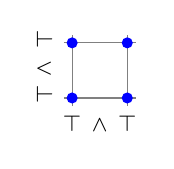
\begin{tikzpicture}[matrix,x=-3.5mm,y=3.5mm]
						\foreach \xs/\ys/\xz/\yz/\xl/\yl/\rot in {0/0/1/0/0/2/90, 0/0/0/1/2/0/0} {
							\foreach \z/\a/\d in {0/\top/1, 1/\wedge/0, 2/\top/1}
								\ifthenelse{\d = 0}{
									\draw[gray] (\xs + \z*\xz - \xl*0.5, \ys + \z*\yz - \yl*0.5)
										node[tgt] {\ifthenelse{\rot > -1}{\rotatebox{\rot}{\footnotesize$\a$}}{}}
										(0,0) -- (0,0)}{
									\draw[gray] (\xs + \z*\xz - \xl*0.5, \ys + \z*\yz - \yl*0.5)
										node[tgt] {\ifthenelse{\rot > -1}{\rotatebox{\rot}{\footnotesize$\a$}}{}}
										(\xs + \z*\xz - \xl*0.15, \ys + \z*\yz - \yl*0.15) -- (\xs + \z*\xz + \xl*1.15, \ys + \z*\yz + \yl*1.15)};};
						\foreach \p/\n/\d in {{0,0}/a1/blue, {0,2}/a2/blue, {2,0}/a3/blue, {2,2}/a4/blue} \node[fill,tok,\d] (\n) at (\p) {};
					\end{tikzpicture}
				\end{minipage}
			\end{minipage}
        \end{minipage}
    }


	
	\frame{
		\frametitle{Datatypes}
		
		Tuple:
		\begin{figure}[H]
    \centering
    \begin{tikzpicture}[every node/.style={scale=0.7}]
        \def\x{1cm}
        \def\y{1cm}
        
        \node[anchor=center](root){};
        \node[on grid, left=       4*\x of root](lroot){};
        \node[on grid, left=       2*\x of lroot  ](13){$(1, 3)$};
        \node[on grid, right=      2*\x of lroot  ](31){$(3, 1)$};
        \node[on grid, below left= \y and \x of 13](23){$(2, 3)$};
        \node[on grid, below right=\y and \x of 13](12){$(1, 2)$};
        \node[on grid, below left= \y and \x of 31](21){$(2, 1)$};
        \node[on grid, below right=\y and \x/2 of 31](32){$(3, 2)$};
        \node[on grid, below right=\y and \x of 12](22){$(2, 2)$};
                        
        \node[on grid, right=      2*\x of root](rroot){};
        \node[on grid, left=       2*\x of rroot  ](57){$(5, 7)$};
        \node[on grid, right=      2*\x of rroot  ](75){$(7, 5)$};
        \node[on grid, below left= \y and \x/2 of 57](67){$(6, 7)$};
        \node[on grid, below right=\y and \x of 57](56){$(5, 6)$};
        \node[on grid, below left= \y and \x of 75](65){$(6, 5)$};
        \node[on grid, below right=\y and \x of 75](76){$(7, 6)$};
        \node[on grid, below right=\y and \x of 56](66){$(6, 6)$};
        
        \node[on grid, below left= \y and 2*\x of 22](224){$(2, 2, 4)$};
        \node[on grid, below left= \y and 0*\x of 22](242){$(2, 4, 2)$};
        \node[on grid, below right=\y and 2*\x of 22](422){$(4, 2, 2)$};
        \node[on grid, below left= \y and 2*\x of 66](466){$(4, 6, 6)$};
        \node[on grid, below left= \y and 0*\x of 66](646){$(6, 4, 6)$};
        \node[on grid, below right=\y and 2*\x of 66](664){$(6, 6, 4)$};
       
        \node[on grid, below left= 2*\y and 3*\x of 22](226){$(2, 2, 6)$};
        \node[on grid, below left= 2*\y and \x of 22  ](262){$(2, 6, 2)$};
        \node[on grid, below right=2*\y and \x of 22  ](622){$(6, 2, 2)$};
        \node[on grid, below left= 2*\y and 3*\x of 66](266){$(2, 6, 6)$};
        \node[on grid, below left= 2*\y and \x of 66  ](626){$(6, 2, 6)$};
        \node[on grid, below right=2*\y and \x of 66  ](662){$(6, 6, 2)$};

        \coordinate[on grid, below=\y of 226   ](246c){};
        \coordinate[on grid, right=2*\x of 246c](264c){};
        \coordinate[on grid, right=2*\x of 264c](426c){};
        \coordinate[on grid, right=2*\x of 426c](462c){};
        \coordinate[on grid, right=2*\x of 462c](624c){};
        \coordinate[on grid, right=2*\x of 624c](642c){};

        \node[on grid, below=\y/2 of 246c](246){$(2, 4, 6)$};
        \node[on grid, below=\y/2 of 264c](264){$(2, 6, 4)$};
        \node[on grid, below=\y/2 of 426c](426){$(4, 2, 6)$};
        \node[on grid, below=\y/2 of 462c](462){$(4, 6, 2)$};
        \node[on grid, below=\y/2 of 624c](624){$(6, 2, 4)$};
        \node[on grid, below=\y/2 of 642c](642){$(6, 4, 2)$};

        \coordinate[on grid, below=2.5*\y of 224](224c){};
        \coordinate[on grid, below=2.5*\y of 242](242c){};
        \coordinate[on grid, below=2.5*\y of 422](422c){};
        \coordinate[on grid, below=2.5*\y of 466](466c){};
        \coordinate[on grid, below=2.5*\y of 646](646c){};
        \coordinate[on grid, below=2.5*\y of 664](664c){};
    
        \coordinate[on grid, below left= 1.5*\y and \x/2 of 224c](244lc){};
        \coordinate[on grid, below right=1.5*\y and \x/2 of 224c](244rc){};
        \coordinate[on grid, below left= 1.5*\y and \x/2 of 242c](424lc){};
        \coordinate[on grid, below right=1.5*\y and \x/2 of 242c](424rc){};
        \coordinate[on grid, below left= 1.5*\y and \x/2 of 422c](442lc){};
        \coordinate[on grid, below right=1.5*\y and \x/2 of 422c](442rc){};
        
        \coordinate[on grid, below left= 1.5*\y and \x/2 of 664c](644lc){};
        \coordinate[on grid, below right=1.5*\y and \x/2 of 664c](644rc){};
        \coordinate[on grid, below left= 1.5*\y and \x/2 of 646c](464lc){};
        \coordinate[on grid, below right=1.5*\y and \x/2 of 646c](464rc){};
        \coordinate[on grid, below left= 1.5*\y and \x/2 of 466c](446lc){};
        \coordinate[on grid, below right=1.5*\y and \x/2 of 466c](446rc){};

        \node[on grid, below=2*\y of 224c](244){$(2, 4, 4)$};
        \node[on grid, below=2*\y of 242c](424){$(4, 2, 4)$};
        \node[on grid, below=2*\y of 422c](442){$(4, 4, 2)$};
        \node[on grid, below=2*\y of 466c](446){$(4, 4, 6)$};
        \node[on grid, below=2*\y of 646c](464){$(4, 6, 4)$};
        \node[on grid, below=2*\y of 664c](644){$(6, 4, 4)$};

        \draw[-arr] (13) to (23);
        \draw[-arr] (13) to (12);
        \draw[-arr] (31) to (21);
        \draw[-arr] (31) to (32);
        \draw[-arr] (23) to (22);
        \draw[-arr] (12) to (22);
        \draw[-arr] (21) to (22);
        \draw[-arr] (32) to (22);
        
        \draw[-arr] (57) to (67);
        \draw[-arr] (57) to (56);
        \draw[-arr] (75) to (65);
        \draw[-arr] (75) to (76);
        \draw[-arr] (67) to (66);
        \draw[-arr] (56) to (66);
        \draw[-arr] (65) to (66);
        \draw[-arr] (76) to (66);        
        
        \drawsquig (22) to (224);
        \drawsquig (22) to (242);
        \drawsquig (22) to (422);
        \drawsquig (66) to (466);
        \drawsquig (66) to (646);
        \drawsquig (66) to (664);

        \drawsquig (22) to (226);
        \drawsquig (22) to (262);
        \drawsquig (22) to (622);
        \drawsquig (66) to (266);
        \drawsquig (66) to (626);
        \drawsquig (66) to (662);

        \draw[-] (226) to (246c) to (266);
        \draw[-] (226) to (426c) to (626);
        \draw[-] (262) to (264c) to (266);
        \draw[-] (262) to (462c) to (662);
        \draw[-] (622) to (624c) to (626);
        \draw[-] (622) to (642c) to (662);

        \draw[-arr] (246c) to (246);
        \draw[-arr] (264c) to (264);
        \draw[-arr] (426c) to (426);
        \draw[-arr] (462c) to (462);
        \draw[-arr] (624c) to (624);
        \draw[-arr] (642c) to (642);

        \draw[-] (224) to (224c);
        \draw[-] (242) to (242c);
        \draw[-] (422) to (422c);
        \draw[-] (466) to (466c);
        \draw[-] (646) to (646c);
        \draw[-] (664) to (664c);

        \draw[-] (246) to (244lc) to (242c);
        \draw[-] (246) to (446lc) to (646c);
        \draw[-] (264) to (244rc) to (224c);
        \draw[-] (264) to (464lc) to (664c);
        \draw[-] (426) to (424lc) to (422c);
        \draw[-] (426) to (446rc) to (466c);
        \draw[-] (462) to (464rc) to (466c);
        \draw[-] (462) to (442lc) to (422c);
        \draw[-] (624) to (644lc) to (664c);
        \draw[-] (624) to (424rc) to (224c);
        \draw[-] (642) to (644rc) to (646c);
        \draw[-] (642) to (442rc) to (242c);

        \draw[-arr] (244lc) to (244);
        \draw[-arr] (424lc) to (424);
        \draw[-arr] (442lc) to (442);
        \draw[-arr] (644lc) to (644);
        \draw[-arr] (464lc) to (464);
        \draw[-arr] (446lc) to (446);
        \draw[-arr] (244rc) to (244);
        \draw[-arr] (424rc) to (424);
        \draw[-arr] (442rc) to (442);
        \draw[-arr] (644rc) to (644);
        \draw[-arr] (464rc) to (464);
        \draw[-arr] (446rc) to (446);

    \end{tikzpicture}
\end{figure}

	}

	\frame{
		\frametitle{Datatypes}

		Multiset:
		\begin{figure}[H]
    \def\x{1cm}
    \def\y{1cm}
    \centering
    \begin{tikzpicture}[every node/.style={scale=0.7}]
        \node[anchor=center](root){};
        \node[on grid, left=       2*\x of root   ](13){$<1, 3>$};
        \node[on grid, right=      2*\x of root   ](57){$<5, 7>$};
        \node[on grid, below left= \y and \x of 13](23){$<2, 3>$};
        \node[on grid, below right=\y and \x of 13](12){$<1, 2>$};
        \node[on grid, below left= \y and \x of 57](67){$<6, 7>$};
        \node[on grid, below right=\y and \x of 57](56){$<5, 6>$};
        \node[on grid, below right=\y and \x of 23](22){$<2, 2>$};
        \node[on grid, below right=\y and \x of 67](66){$<6, 6>$};

        \node[on grid, below left= \y and \x of 22](224){$<2, 2, 4>$};
        \node[on grid, below right=\y and \x of 22](226){$<2, 2, 6>$};
        \node[on grid, below left= \y and \x of 66](266){$<2, 6, 6>$};
        \node[on grid, below right=\y and \x of 66](466){$<4, 6, 6>$};

        \coordinate[on grid, right=\x of 226](246c){};
        \node[on grid, below right=\y and \x of 226](246){$<2, 4, 6>$};
        \coordinate[on grid, left =2*\x of 246](244c){};
        \node[on grid, below left =\y and \x of 246](244){$<2, 4, 4>$};
        \coordinate[on grid, right=2*\x of 246](446c){};
        \node[on grid, below right=\y and \x of 246](446){$<4, 4, 6>$};
        \coordinate[on grid, below=\y of 246](444c){};
        \node[on grid, below right=\y and \x of 244](444){$<4, 4, 4>$};

        \draw[-arr] (13) to (23);
        \draw[-arr] (13) to (12);
        \draw[-arr] (57) to (67);
        \draw[-arr] (57) to (56);
        \draw[-arr] (23) to (22);
        \draw[-arr] (12) to (22);
        \draw[-arr] (67) to (66);
        \draw[-arr] (56) to (66);

        \drawsquig (22) to (224);
        \drawsquig (22) to (226);
        \drawsquig (66) to (266);
        \drawsquig (66) to (466);

        \draw[-] (226) to (246c) to (266);
        \draw[-] (224) to (244c) to (246);
        \draw[-] (466) to (446c) to (246);
        \draw[-] (244) to (444c) to (446);
        
        \draw[-arr] (246c) to (246);
        \draw[-arr] (244c) to (244);
        \draw[-arr] (446c) to (446);
        \draw[-arr] (444c) to (444);
    \end{tikzpicture}
\end{figure}


		\begin{itemize}
            \item Store tokens as sorted tuples
            \item Matrix is upper-triangular (in n-dimensions)
		\end{itemize}
	}


	\frame{
		\frametitle{Datatypes}
		
		Set:
		\begin{figure}[H]
    \centering
    \begin{tikzpicture}
        \def\x{1cm}
        \def\y{1cm}
        
        \node[anchor=center](root){};
        \node[on grid, left=       2*\x of root   ](13){$\{1, 3\}$};
        \node[on grid, right=      2*\x of root   ](57){$\{5, 7\}$};
        \node[on grid, below left= \y and \x of 13](23){$\{2, 3\}$};
        \node[on grid, below right=\y and \x of 13](12){$\{1, 2\}$};
        \node[on grid, below left= \y and \x of 57](67){$\{6, 7\}$};
        \node[on grid, below right=\y and \x of 57](56){$\{5, 6\}$};
        \node[on grid, below right=\y and \x of 23](2){$\{2\}$};
        \node[on grid, below right=\y and \x of 67](6){$\{6\}$};
        \coordinate[on grid, right=2*\x of 2](4c){};
        \node[on grid, below right=\y and 2*\x of 2](4){$\{4\}$};

        \draw[-arr] (13) to (23);
        \draw[-arr] (13) to (12);
        \draw[-arr] (57) to (67);
        \draw[-arr] (57) to (56);
        \draw[-arr] (23) to (2);
        \draw[-arr] (12) to (2);
        \draw[-arr] (67) to (6);
        \draw[-arr] (56) to (6);
        \draw[-] (2) to (4c) to (6);
        \draw[-arr] (4c) to (4);
    \end{tikzpicture}
\end{figure}

	}
	
\frame{
		\frametitle{Datatypes}
		
		Set:
		\begin{figure}[H]
    \def\x{1cm}
    \def\y{0.7cm}
    \centering
    \begin{tikzpicture}[every node/.style={scale=0.7}]
        \node[anchor=center](root){};
        \node[on grid, left=       2*\x of root   ](13){$\{a, \neg a\}$};
        \node[on grid, right=      2*\x of root   ](57){$\{b, \neg b\}$};
        \node[on grid, below left= \y and \x of 13](23){$\{a \vee \neg a, \neg a\}$};
        \node[on grid, below right=\y and \x of 13](12){$\{a, a \vee \neg a\}$};
        \node[on grid, below left= \y and \x of 57](67){$\{b \vee \neg b, \neg b\}$};
        \node[on grid, below right=\y and \x of 57](56){$\{b, b \vee \neg b\}$};
        \node[on grid, below right=\y and \x of 23](2){$\{a \vee \neg a\}$};
        \node[on grid, below right=\y and \x of 67](6){$\{b \vee \neg b\}$};
        \coordinate[on grid, below right=0.5*\y and 2*\x of 2](4c){};
        \node[on grid, below=0.5*\y of 4c](4){$\{(a \vee \neg a) \wedge (b \vee \neg b)\}$};

        \draw[-arr] (13) to (23);
        \draw[-arr] (13) to (12);
        \draw[-arr] (57) to (67);
        \draw[-arr] (57) to (56);
        \draw[-arr] (23) to (2);
        \draw[-arr] (12) to (2);
        \draw[-arr] (67) to (6);
        \draw[-arr] (56) to (6);
        \draw[-] (2) to (4c) to (6);
        \draw[-arr] (4c) to (4);
    \end{tikzpicture}
\end{figure}

		
		\begin{itemize}
			\item How should the matrix be encoded?
		\end{itemize}
	}


	\frame{
        \frametitle{Dimensionality}
		
		\begin{align*}
			\mathcal{D}^1 \quad \defeq \quad &\top \mid \bot \mid \mathcal{D}^1 \vee \mathcal{D}^1 \mid \mathcal{D}^1 \wedge \mathcal{D}^1 \\
			\mathcal{D}^2 \quad \defeq \quad &ALL \mid A \vee \dual A \mid \mathcal{D}^{n \le 2} \wedge \mathcal{D}^2 \mid \mathcal{D}^{n \ge 2} \vee \mathcal{D}^2 \\
			\mathcal{D}^3 \quad \defeq \quad &(A \wedge B) \vee (\dual A \wedge B) \vee (A \wedge \dual B) \vee (\dual A \wedge \dual B) \\
										     &\mid \mathcal{D}^{n \le 3} \wedge \mathcal{D}^3 \mid \mathcal{D}^{n \ge 3} \vee \mathcal{D}^3 \\
				          		\dots  \quad &
		\end{align*}

		\begin{itemize}
			\item $A \in \mathcal{D}^n, B \in \mathcal{D}^m$ $\implies$ $A \vee B \in \mathcal{D}^{min(n, m)}$, $A \wedge B \in \mathcal{D}^{max(n, m)}$
		\end{itemize}
    }



    \frame{
        \frametitle{Dimensionality Bounds}
		
		\begin{itemize}
			\item Number of variables
			\item Dimensionality of largest \emph{disjunctive normal form} term
			\item Exact bound is equivalent to proof search?
		\end{itemize}
    }



    \frame{
        \frametitle{Questions?}

        
    }



    \frame{
        \frametitle{References}

        \bibliography{dortmund}
    }

\end{document}
